\documentclass[12pt,english,letterpaper]{scrartcl}
\usepackage[top=1in, bottom=1in, left=1.25in, right=1.25in]{geometry}

\usepackage{graphicx}
\usepackage[unicode=true,pdfusetitle,
bookmarks=true,bookmarksnumbered=false,bookmarksopen=false,
breaklinks=true,pdfborder={0 0 1},backref=false,colorlinks=true]
{hyperref}
\hypersetup{
	urlcolor=blue,linkcolor=blue}
\usepackage{pdfpages}
\usepackage{indentfirst}

\title{Additional Documentation in Support of Permit Application P526-190319-001}
\author{Prepared by Aubrey Moore PhD, Entomologist, University of Guam}
\date{June 2, 2019}

\begin{document}

\maketitle

\tableofcontents

\section{Background and Justification}
On March 19, 2019 I requested a permit to import live coconut rhinoceros beetles (CRB), \textit{Oryctes rhinoceros}, to Guam (Application number P526-190319-001) to replace permit P526P-11-01844 for this purpose (Appendix \ref{old permit}), which I accidentally allowed to lapse into oblivion after only one shipment.

On May 10, 2019 I was sent automated email from the USDA-APHIS permit office requesting additional information in the form of an Applicant Inspection Questionnaire. This document is a response to that request.

I request permission to import live coconut rhinoceros beetles, \textit{Oryctes rhinoceros}, into Guam. These beetles will be used in USDA-APHIS funded laboratory research aimed at developing biological control for this species. No imported beetles or their progeny will be released on Guam.

Massive mortality of coconut and other palms is occurring on Guam and several other Pacific islands as the result of uncontrolled outbreaks of coconut rhinoceros beetle biotype G (CRB-G). Pacific island invasions of CRB where previously controlled by a microbial biological control agent, \textit{Oryctes rhinoceros} nudivirus (OrNV). Unfortunately, CRB-G appears to be resistant to all currently available isolates of OrNV. My laboratory is funded by USDA-APHIS Farm Bill grants to
find new isolates of OrNV which can be used for effective biological control of CRB-G. We are importing OrNV samples under Import Permit P526P-17-03146 and are evaluating these as potential biological control agents in laboratory bioassays. 

We have established a laboratory colony of CRB-G to supply insects for bioassays. But we also need to establish a laboratory colony of virus-susceptible beetles for our tests. We request permission to import beetles from foreign sources because CRB-G is the only biotype known to exist on Guam.

%We request that you attach your Standard Operating Procedure (SOP) using the "Facility Attachments" hyperlink. For directions on what should be included in your SOP go to:
%
%http://www.aphis.usda.gov/plant_health/permits/organism/containment_facility_inspections.shtml
%
%
%
%
%
%http://www.aphis.usda.gov/plant_health/permits/organism/containment_facility_inspections.shtml
%
%is redirected to:
%
%https://www.aphis.usda.gov/aphis/ourfocus/planthealth/import-information/permits
%
%
%Questionnaire general comments.
%
%
%
%Please provide electronic photographs of cages, rooms that will be used and insects housed including doors with door sweeps, autoclave, i.e., all relevant safeguards that are in place to ensure adequate containment of the regulated organisms. We will make our assessments based on this answers to the questionnaire and photos provided, please send us all material that will help us to understand your facility and how you plan to manage the organisms requested.

\section{Quarantine Facility}

The University of Guam operates a USDA Biological Control Facility in House 35, Dean's Circle, University of Guam Campus, Mangilao. I am not intending to use this facility for my project. Instead, I request permission to contain beetles in room 319, Agriculture and Life Sciences Bldg, University of Guam Campus, Mangilao because:
\begin{itemize}
	\item The House 35 site does not have environmental chambers required for establishment and containment of a laboratory colony and for containment of insects during bioassays. 
	\item If beetles were kept in the House 35 facility, this would require carrying beetles outdoors between buildings in order to perform bioassays and to make daily observations. 
\end{itemize}

\section{Standard Operating Procedures}

\subsection{Compliance} 
All conditions specified in permit will be met.
	
\subsection{Transportation}
We have developed a highly secure container for shipment of CRB (Appendix \ref{shipping container}). This container will be used for all shipments.

All packing material and insect bedding material (peat moss) will be autoclaved prior to final disposal.
	  	
\subsection{Rearing conditions}
Imported CRB will be reared individually in Mason jars enclosed by metal caps Fig. \ref{fig:jars}.
\begin{figure}[h]
	\centering
	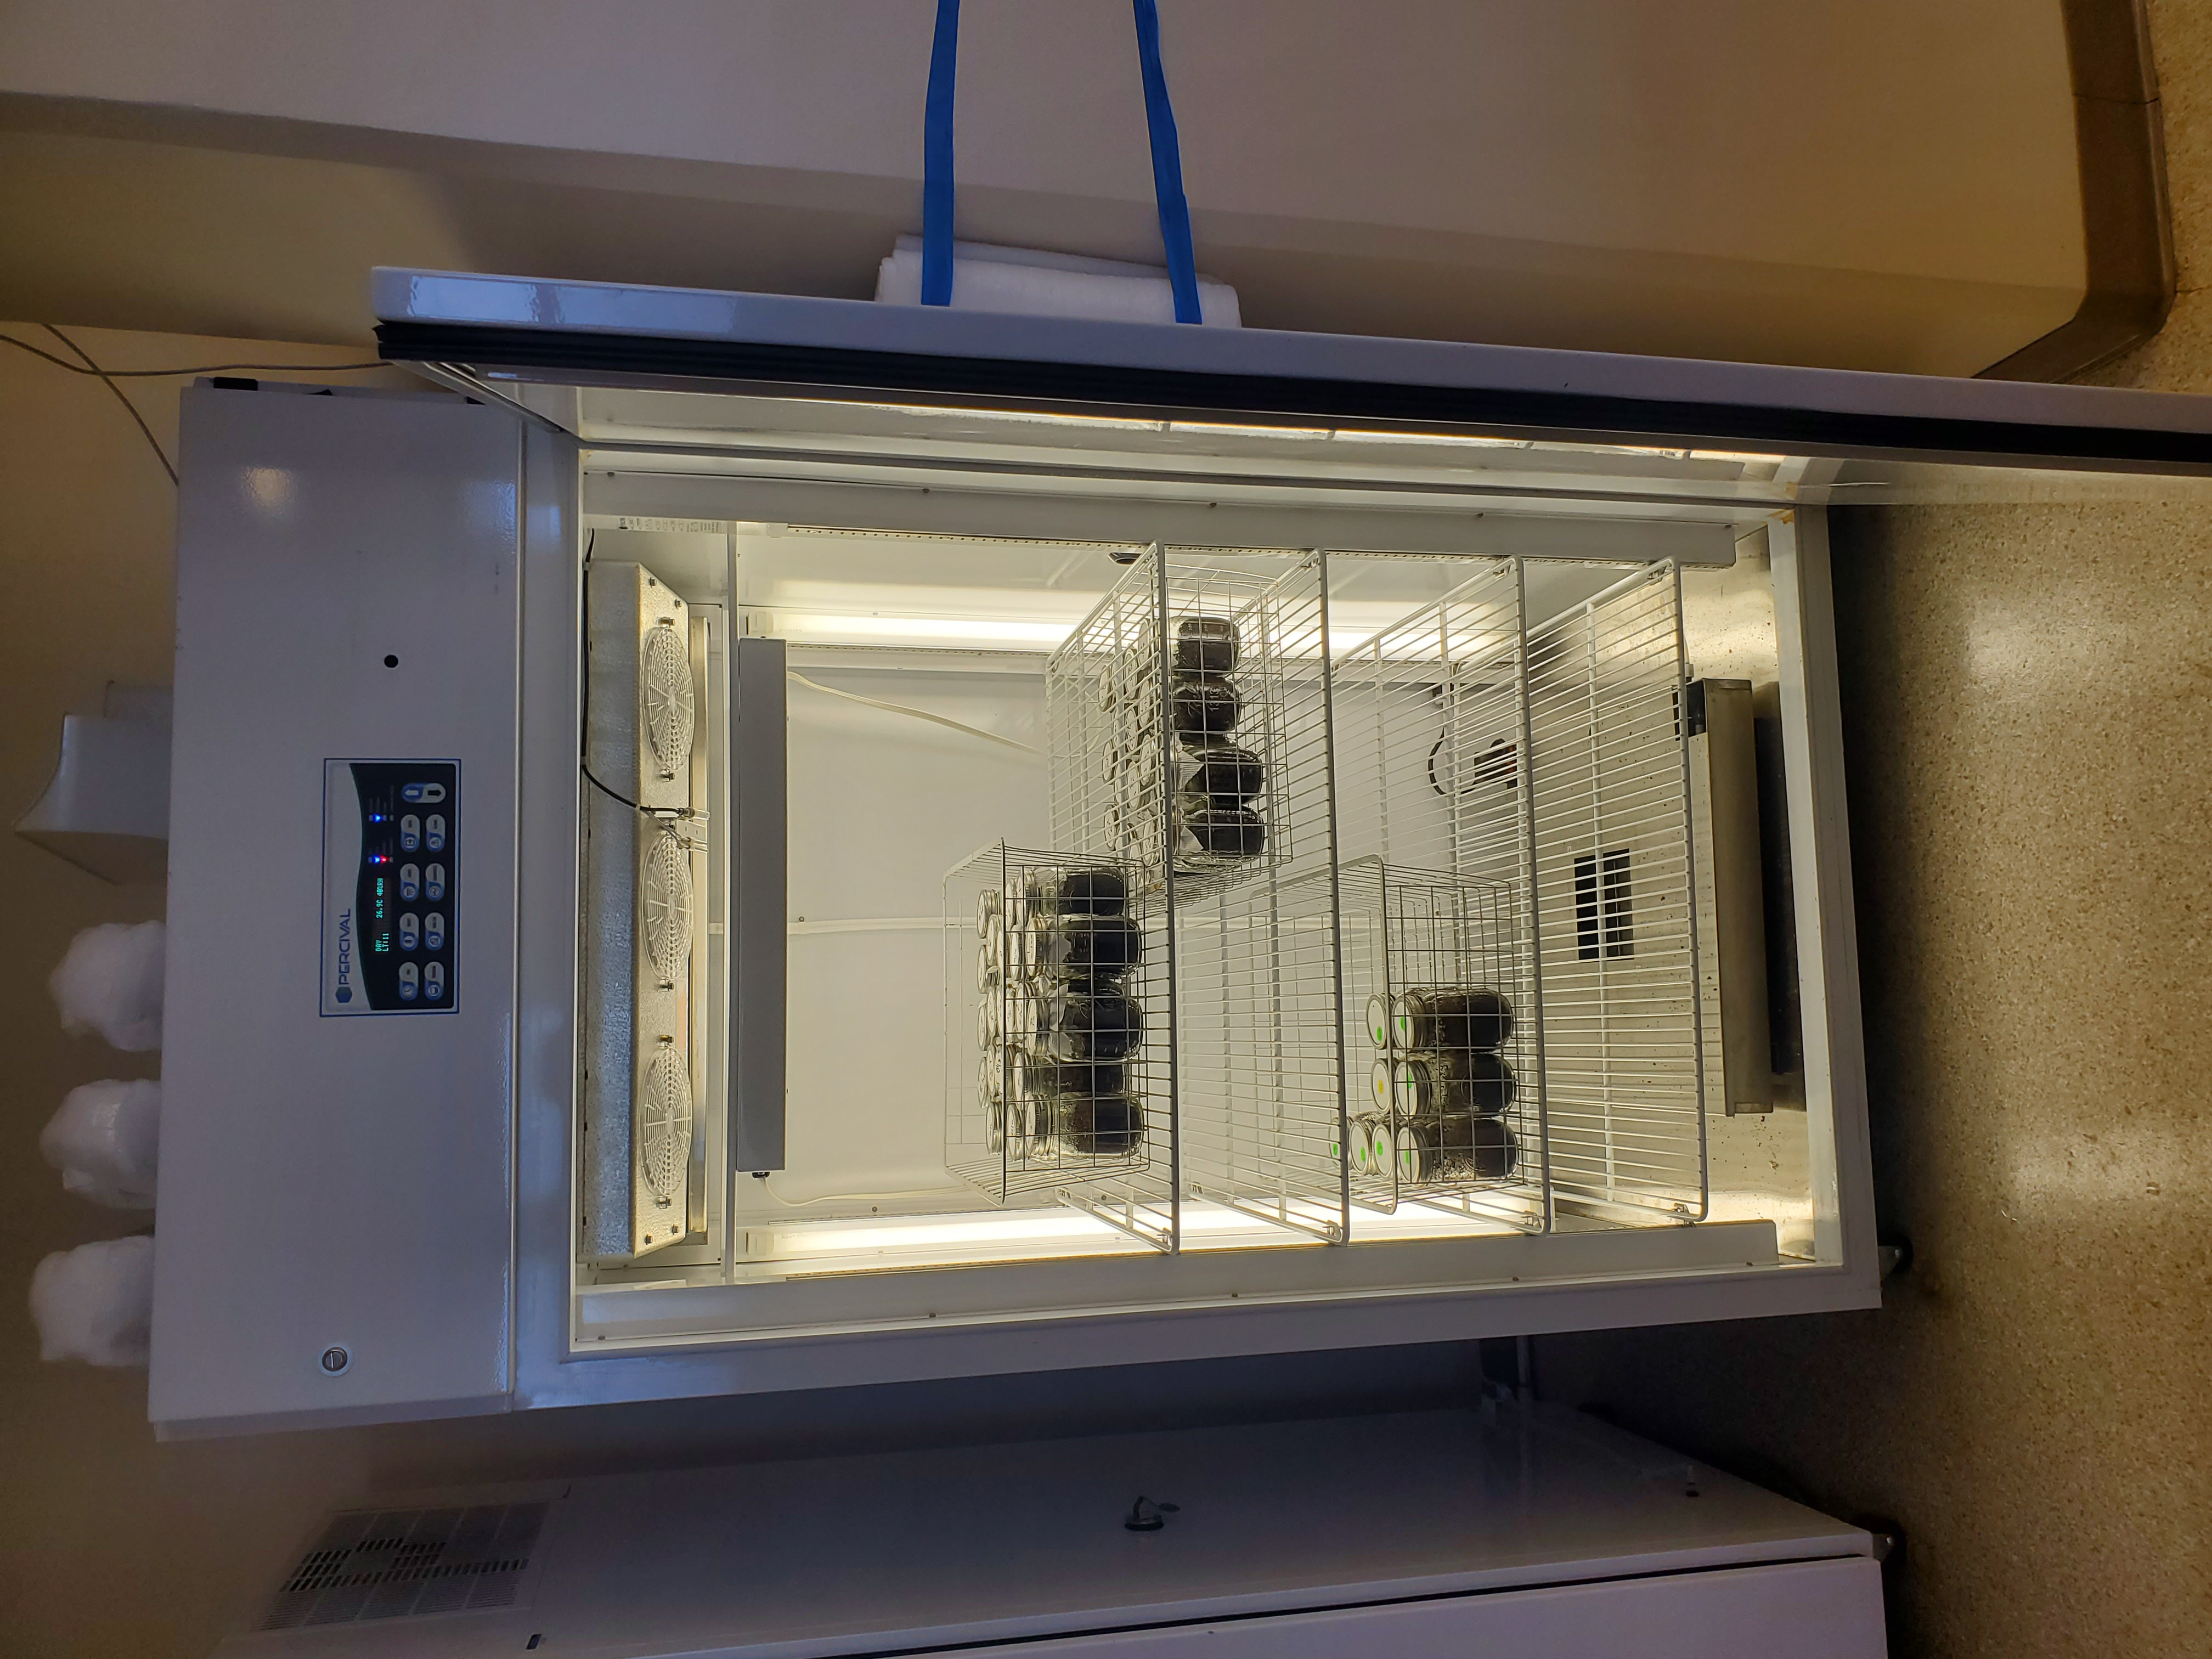
\includegraphics[width=\textwidth, angle =-90]{jars.jpg}
	\caption{CRB are reared individually, in Mason jars with metal caps.}
	\label{fig:jars}
\end{figure}

Mason jars will be in environmental cabinets in a locked room with sealed windows (Room 319, Agricultural and Life Sciences Building, University of Guam, Mangilao, Guam)Fig. \ref{fig:cabinets}.
\begin{figure}[h]
	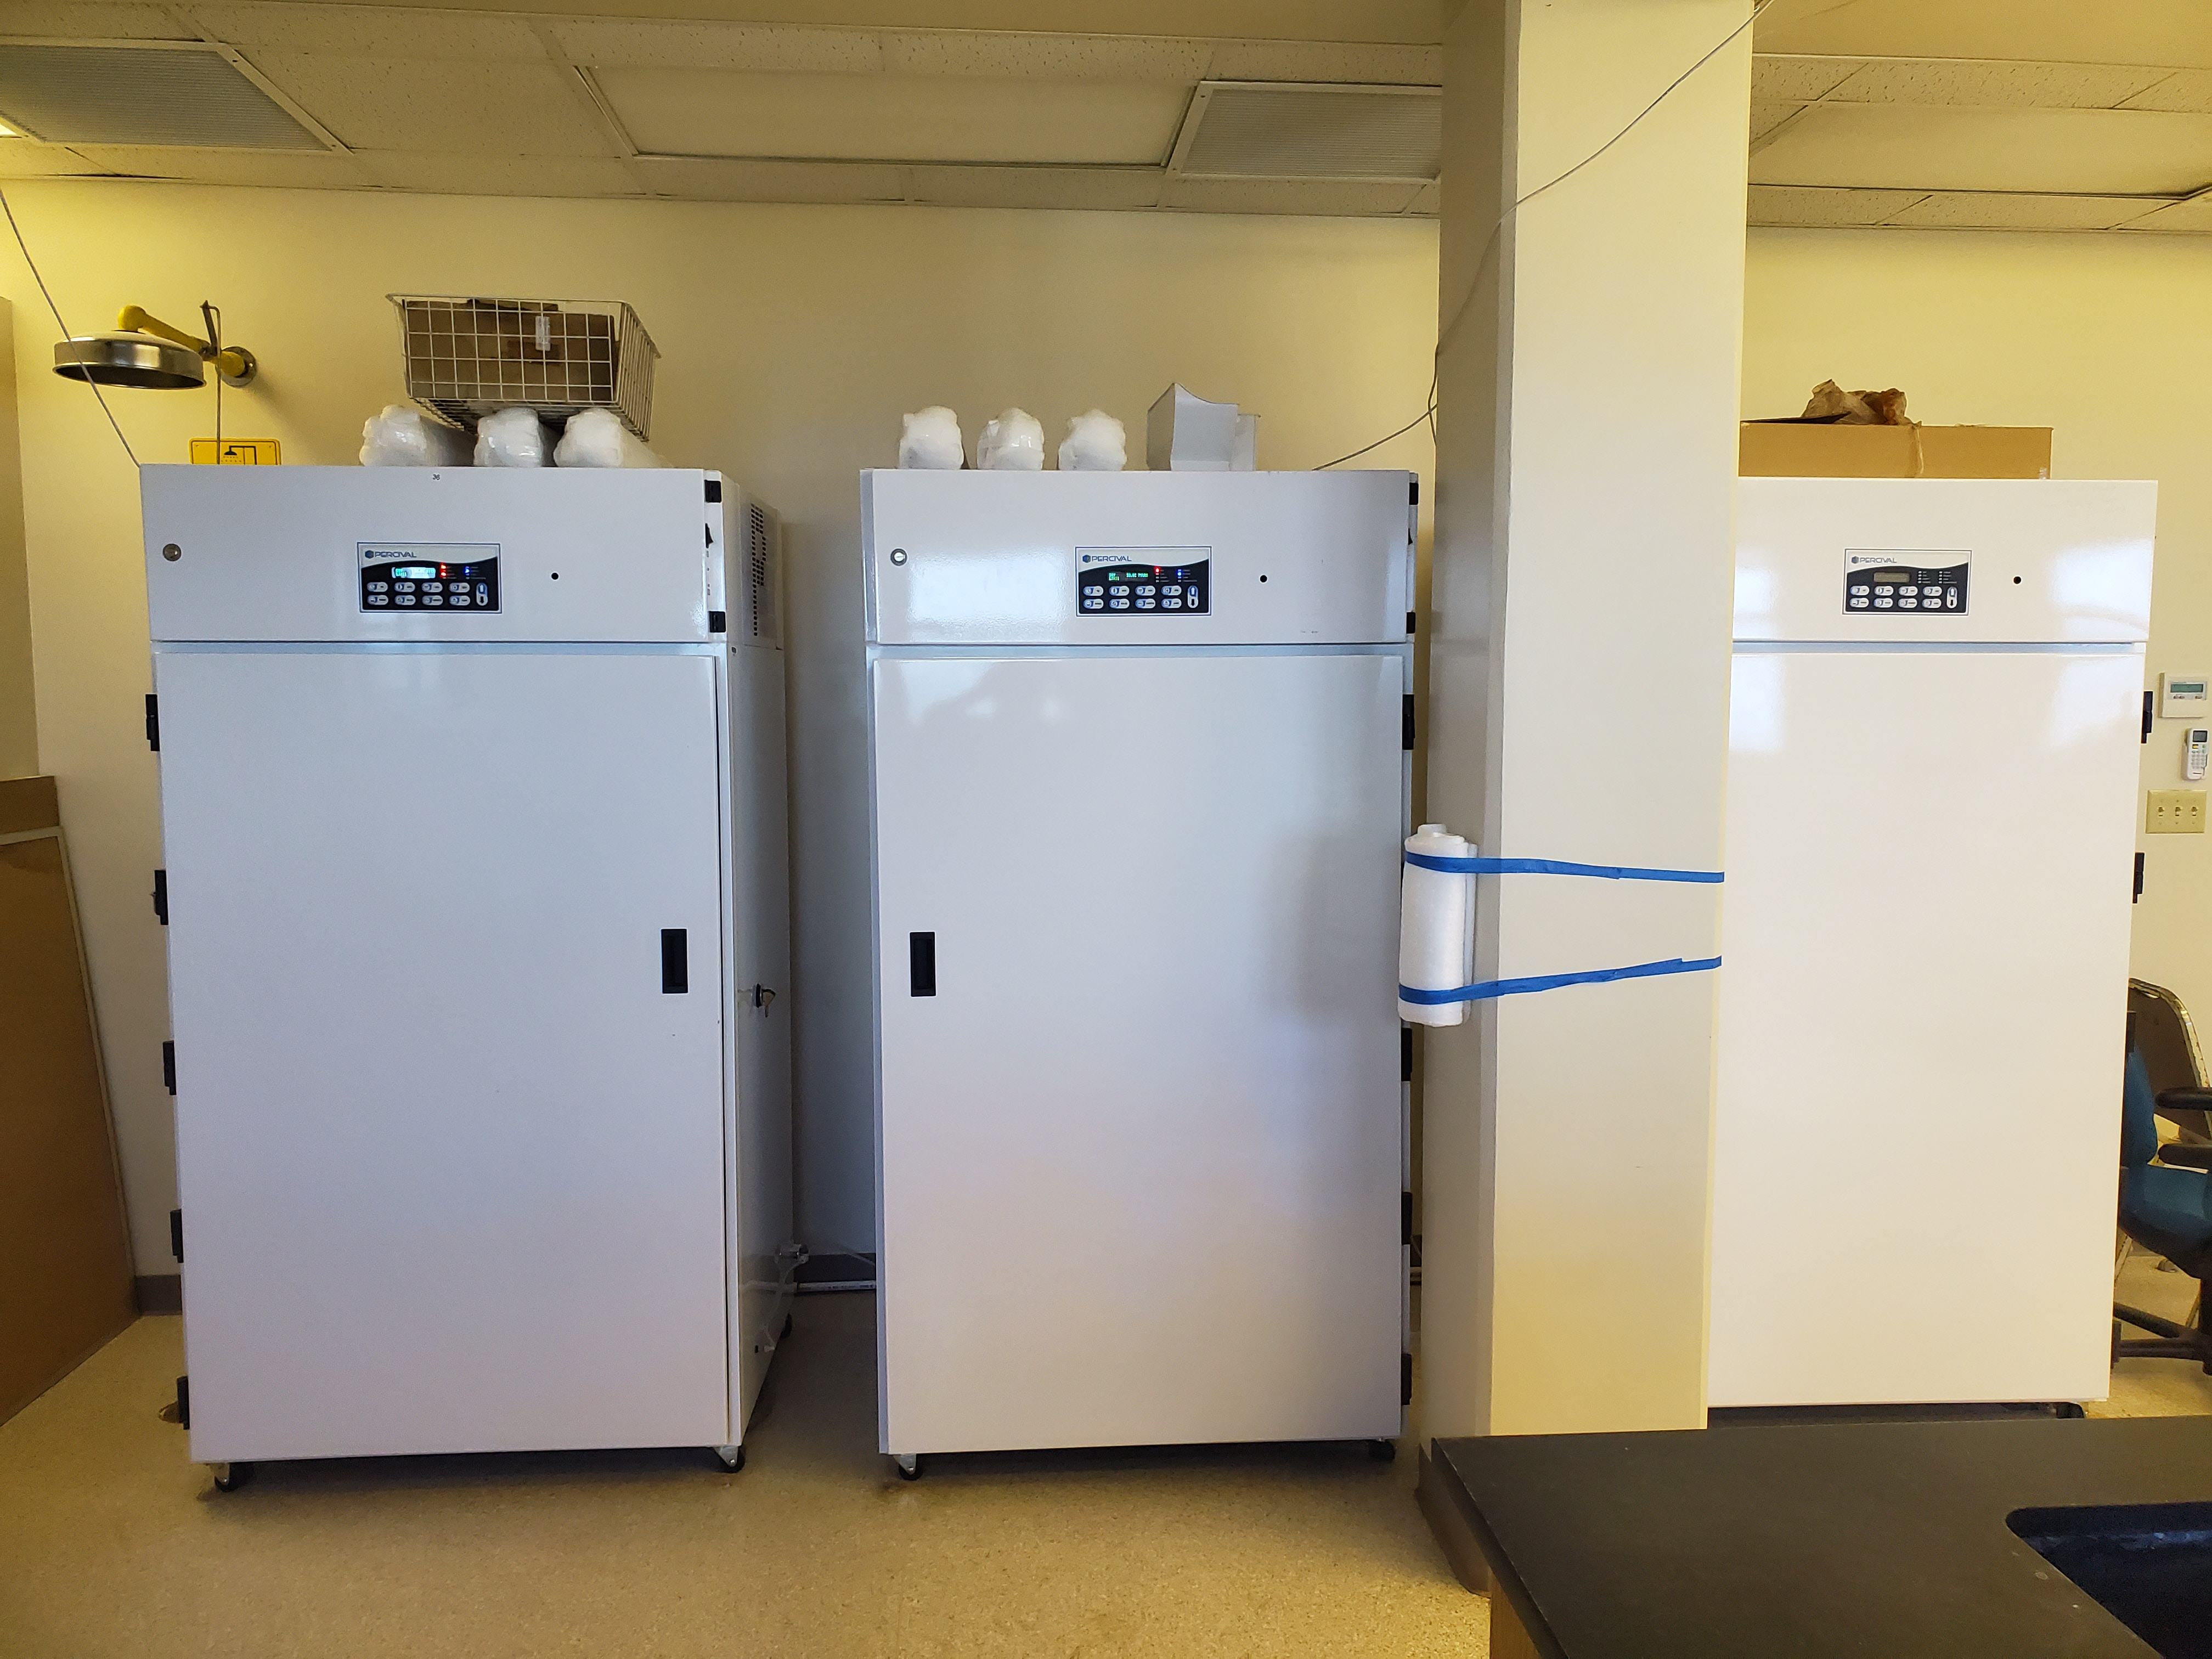
\includegraphics[width=\textwidth]{cabinets.jpg}
	\caption{Environmental cabinets in Room 319, Agricultural and Life Sciences Building, University of Guam, Mangilao, Guam.}
	\label{fig:cabinets}
\end{figure}
	
\subsection{Record keeping}
Detailed records for each individual beetle will be stored in an on existing online laboratory information management system (LIMS). These data will be made available to USDA-APHIS.

\section{Note on Risk}

CRB are very large scarab beetles and are more easily contained than smaller insects which can pass through small openings such gaps around doors. Our beetles are kept individually inside sealed Mason jars inside sealed environmental chambers inside a locked room. If the suggested containment protocol is followed, it is very unlikely that any beetles will escape into the Guam environment. However even if foreign CRB escaped and started to breed, this would not measurably increase damage beyond what is already present on Guam (Fig. \ref{fig:damage}).

\begin{figure}[h]
	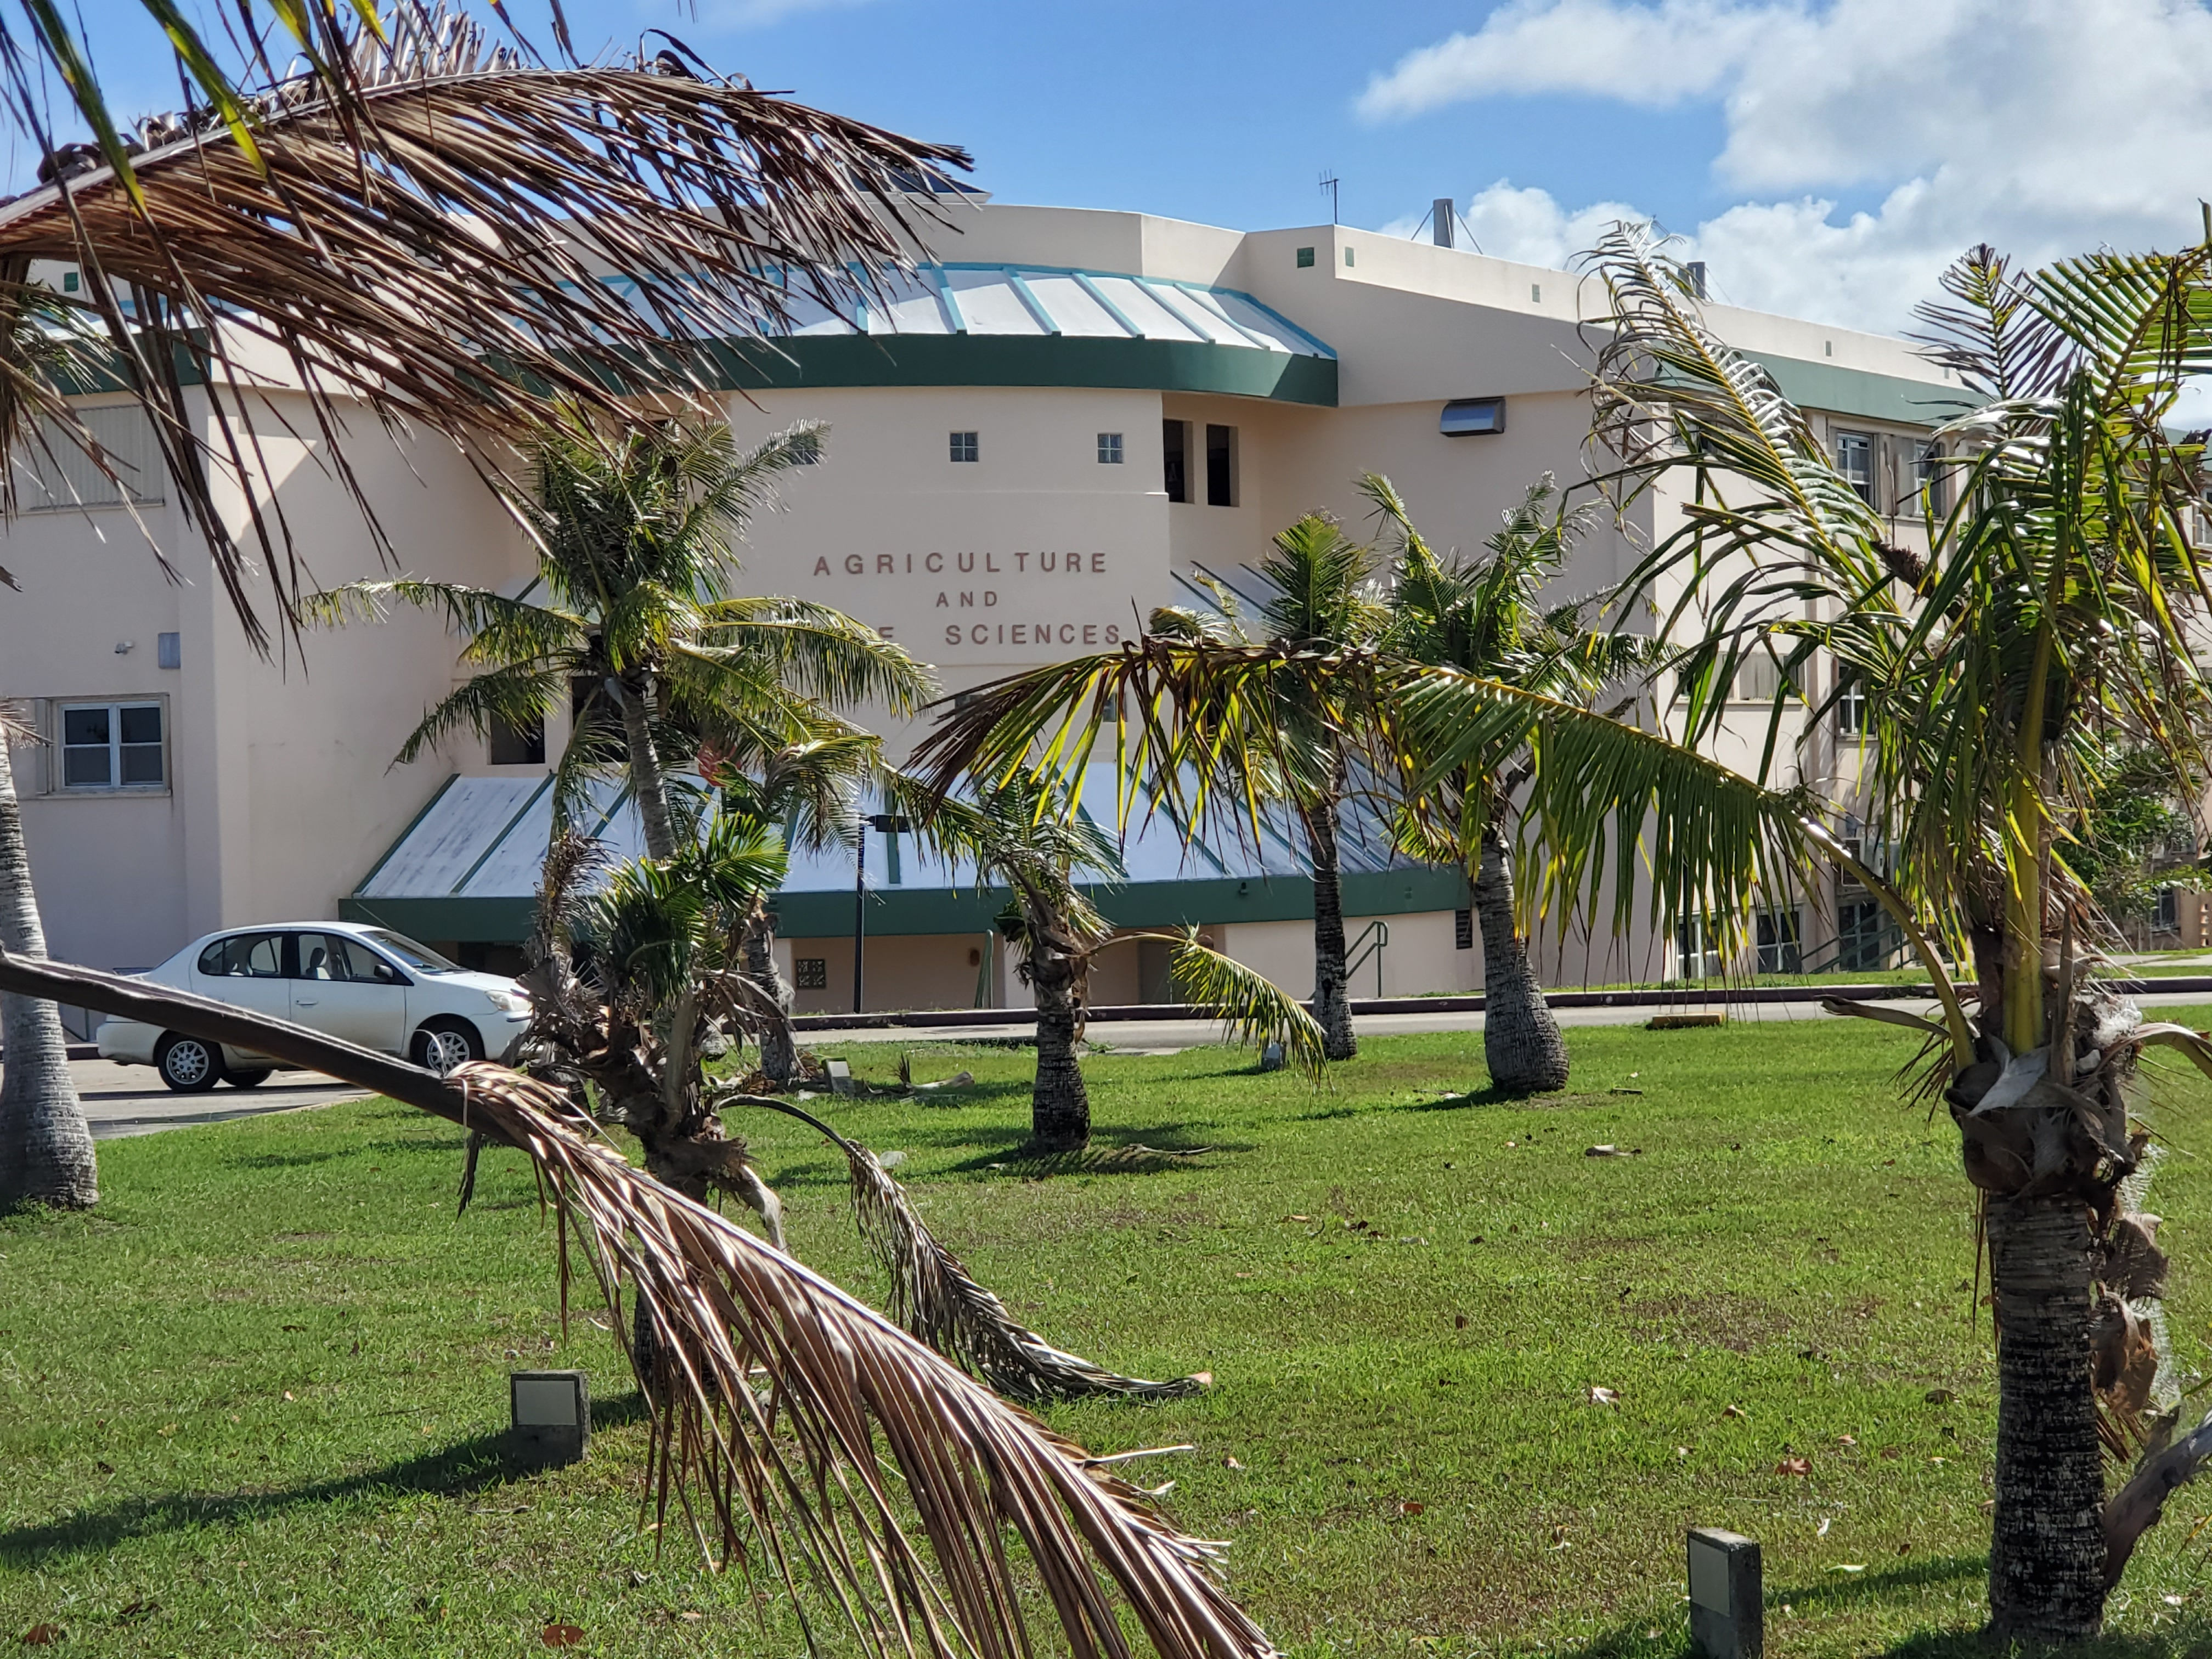
\includegraphics[width=\textwidth]{damage.jpg}
	\caption{Damage}
	\label{fig:damage}
\end{figure}

\clearpage
\appendix
\section{Expired Permit to Import Coconut Rhinoceros Beetles P526P-11-01844}\label{old permit}
Please see next page.

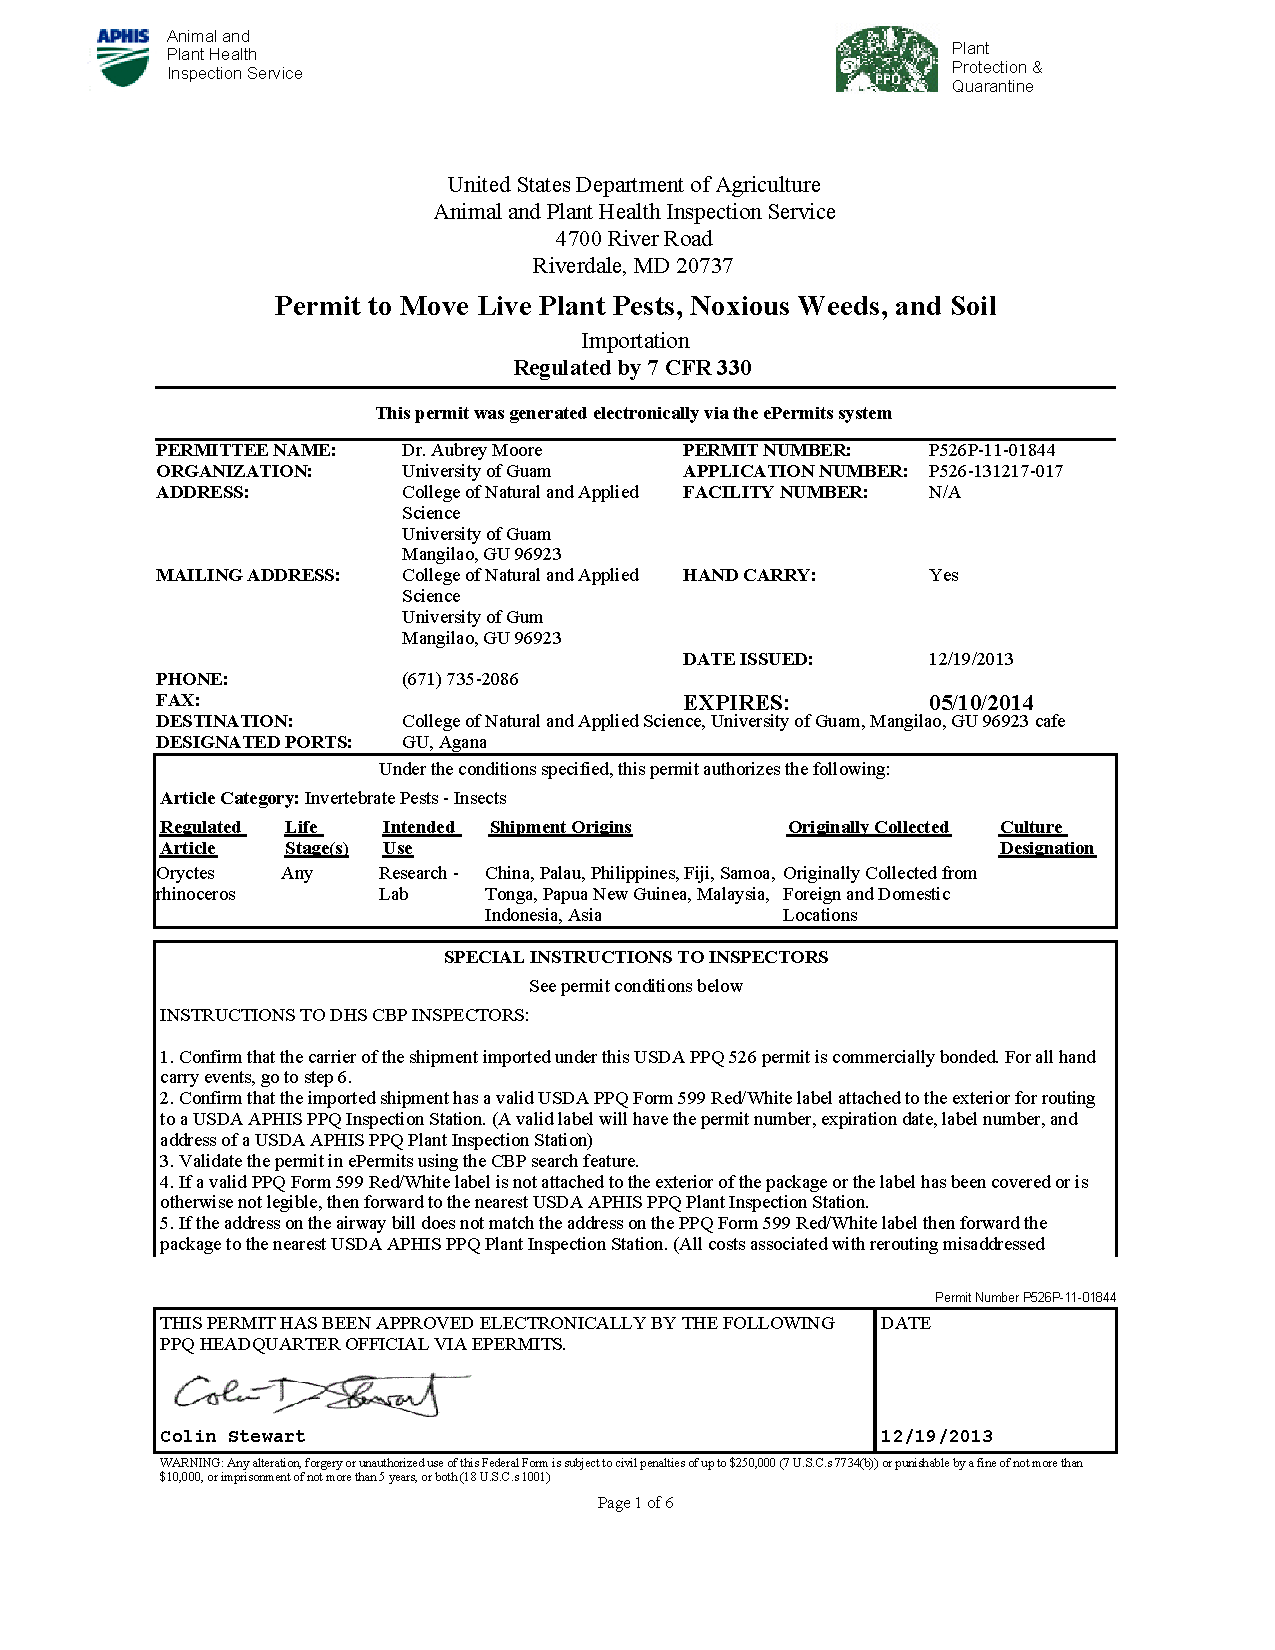
\includepdf[pages=-]{CRB-Import-Permit-P526P-11-01844}

\section{Secure CRB Shipping Container}\label{shipping container}
Please see next page.
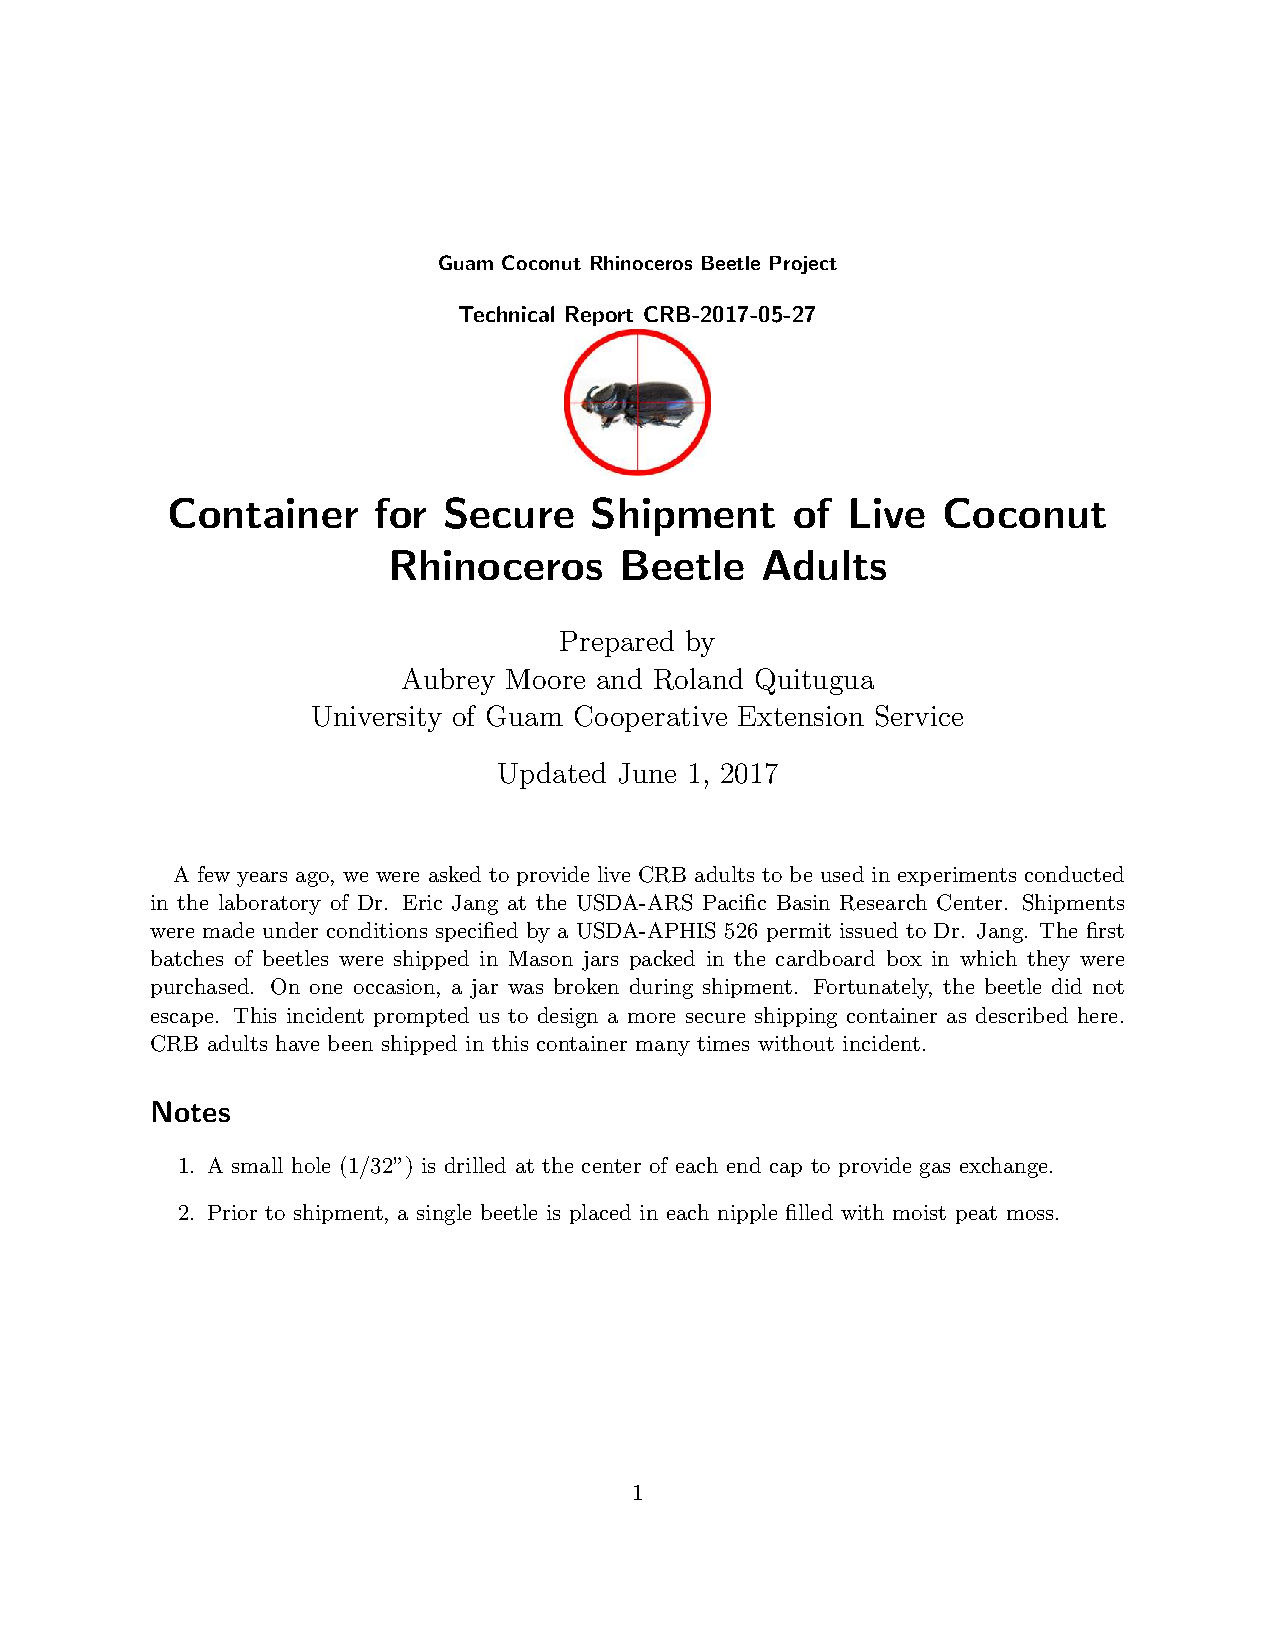
\includepdf[pages=-]{CRB_Shipping_Container}

\end{document}
